\chapter{Исследовательская часть}

В данном разделе поставлена задача исследования зависимости времени выполнения запросов от объема данных в базе данных с наличием или без наличия в базе данных индекса для соответствующего атрибуты таблицы.

В дополнение к этому, представлены технические характеристики устройства, на котором были проведены измерения времени выполнения программного обеспечения, а также результаты измерений, отображенные в виде таблиц и графиков.

\section{Технические характеристики}

При проведении исследования системы важно учитывать характеристики устройства, на котором проводятся измерения, поскольку численные результаты могут различаться в зависимости от конкретных параметров данного устройства.
Технические характеристики этого устройства, на котором проводилось исследование.
\begin{itemize}
	\item Процессор: Intel(R) Core(TM) i5-10300H CPU 2.50 ГГц~\cite{intel}.
	\item Количество ядре: 4 физических и 8 логических ядер.
	\item Оперативная память: 16 ГБайт.
	\item Операционная система: Windows 11 Pro 64-разрядная система~\cite{windows}.
\end{itemize}

Исследование проводилось на стационарном компьютере. Во время тестирования устройство было нагружено только встроенными приложениями окружения.

\section{Постановка задачи исследования}

Индекс~\cite{indexsql} в базе данных --- это структура данных, которая помогает сократить время поиска запрошенных данных. Индексы достигают этого за счет дополнительных затрат на хранение, память и поддержание их в актуальном состоянии, что приводит к повышению времени выполнения операций вставки, изменения и удаления.

Целью исследования является изучение зависимости времени выполнения запросов от объема данных в базе данных от наличия соответствующего индекса базы данных.

Для исследования были выбраны: сущность <<зона>>, по той причине, что сущность имеет отношение многие ко многим к сущности <<пакет>> и один ко многим к сущности <<инвентарь>>, а также сущности <<брони>>, по той причине что она имеет связи один ко многим к сущностям <<зона>>, <<пакета>>, <<пользователь>>. Таким образом для исследования были выбраны следующие запросы.
\begin{enumerate}
	\item Запрос для получение всех данных о зонах, включая информацию о пакетах и инвентаре для конкретной зоны. Реализация данного запроса представлена на листинге~\ref{lst:research-1}.
	\item Запрос на получение всех данных броней. Реализация данного запроса представлена на листинге~\ref{lst:research-2}.
	\item Запрос на получение всех данных броней по идентификатору пользователя. Реализация данного запроса представлена на листинге~\ref{lst:research-3}.
\end{enumerate}

\begin{center}
	\begin{lstlisting}[label=lst:research-1, caption=Запрос на получение всех зон включая информацию пакетах и инвентаре]
public Task<List<Zone>> GetAllZonesAsync(Role role)
{
	return _contextFactory.GetDbContext(role).Zones
	.Include(z => z.Inventories)
	.Include(z => z.Packages).AsNoTracking()
	.Select(z => ZoneConverter.ConvertDbModelToAppModel(z))
	.ToListAsync();
}
	\end{lstlisting}
\end{center}

\begin{center}
	\begin{lstlisting}[label=lst:research-2, caption=Запрос на получение всех броней]
public Task<List<Booking>> GetAllBookingAsync(Role role)
{
	return 
	_contextFactory.GetDbContext(role)
	.Bookings
	.OrderBy(b => b.Date)
	.Select(b => BookingConverter.ConvertDbModelToAppModel(b))
	.ToListAsync();
}
	\end{lstlisting}
\end{center}

\begin{center}
	\begin{lstlisting}[label=lst:research-3, caption=Запрос на получение броней пользователя]
public Task<List<Booking>> GetBookingByUserAsync(Guid userId, Role role) 
{
	return _contextFactory.GetDbContext(role)
	.Bookings.Where(b => b.UserId == userId)
	.OrderBy(b => b.Date)
	.Select(b => BookingConverter.ConvertDbModelToAppModel(b))
	.ToListAsync();
}
	\end{lstlisting}
\end{center}

Исследование проводилось для состояний таблицы зон содержащих от 10 до 10000 записей в таблице.

\section{Сравнение времени обработки}

В таблицах~\ref{tbl:time-1}--\ref{tbl:time-2} продемонстрировано время выполнения запросов с использованием индекса и без него.

На рисунках~\ref{grafics:research-1}--\ref{grafics:research-3} представлены графики зависимости времени выполнения от объема полученных результатов.

\clearpage

\begin{table}[ht]
	\small
	\begin{center}
		\begin{threeparttable}
			\caption{Зависимость времени выполнения запроса на получение данных зон}
			\label{tbl:time-1}
			\begin{tabular}{|c|c|c|}
				\hline
				\multirow{2}{*}{\bfseries Количество записей в таблице зон} & \multicolumn{2}{c|}{\bfseries Время, мс} \\ \cline{2-3}
				& \bfseries Без индексов & \bfseries С индексами
				\csvreader{csv/research-1.csv}{}
				{\\\hline \csvcoli & \csvcolii & \csvcoliii } \\
				\hline
			\end{tabular}
		\end{threeparttable}
	\end{center}
\end{table}

\begin{figure}[h]
	\centering
	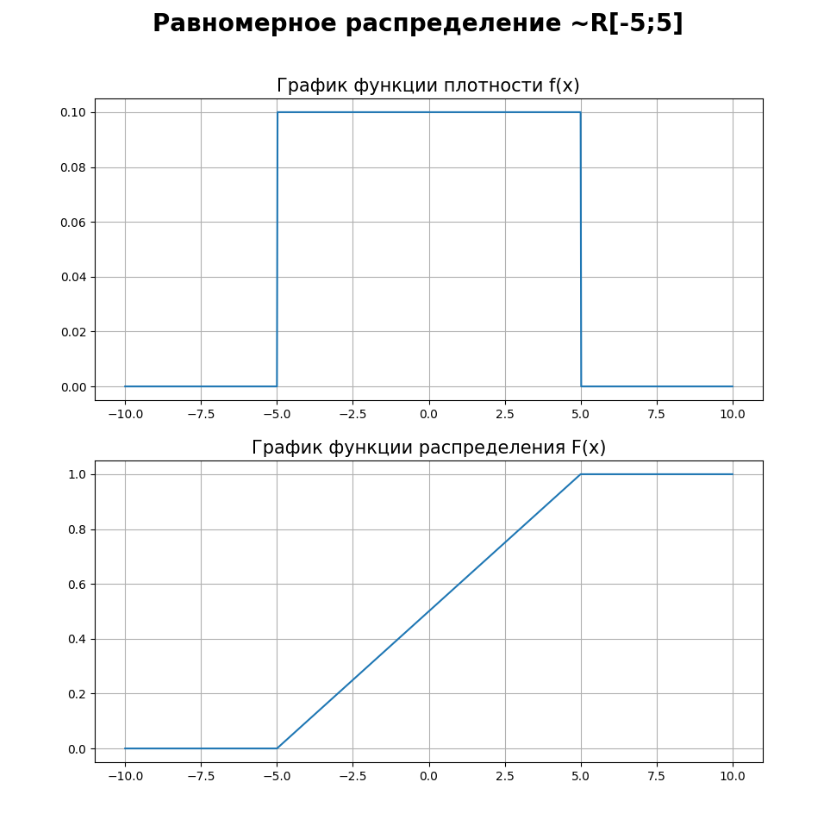
\includegraphics[width=0.6\textwidth]{img/r1.png}
	\caption{График зависимости времени выполнения запроса на получение данных зон}
	\label{grafics:research-1}
\end{figure}

\clearpage

\begin{table}[ht]
	\small
	\begin{center}
		\begin{threeparttable}
			\caption{Зависимость времени выполнения запроса от количества всех броней}
			\label{tbl:time-2}
			\begin{tabular}{|c|c|c|}
				\hline
				\multirow{2}{*}{\bfseries Количество записей в таблице броней} & \multicolumn{2}{c|}{\bfseries Время, мс} \\ \cline{2-3}
				& \bfseries Без индексов & \bfseries С индексами
				\csvreader{csv/research-2.csv}{}
				{\\\hline \csvcoli & \csvcolii & \csvcoliii } \\
				\hline
			\end{tabular}
		\end{threeparttable}
	\end{center}
\end{table}

\begin{figure}[h]
	\centering
	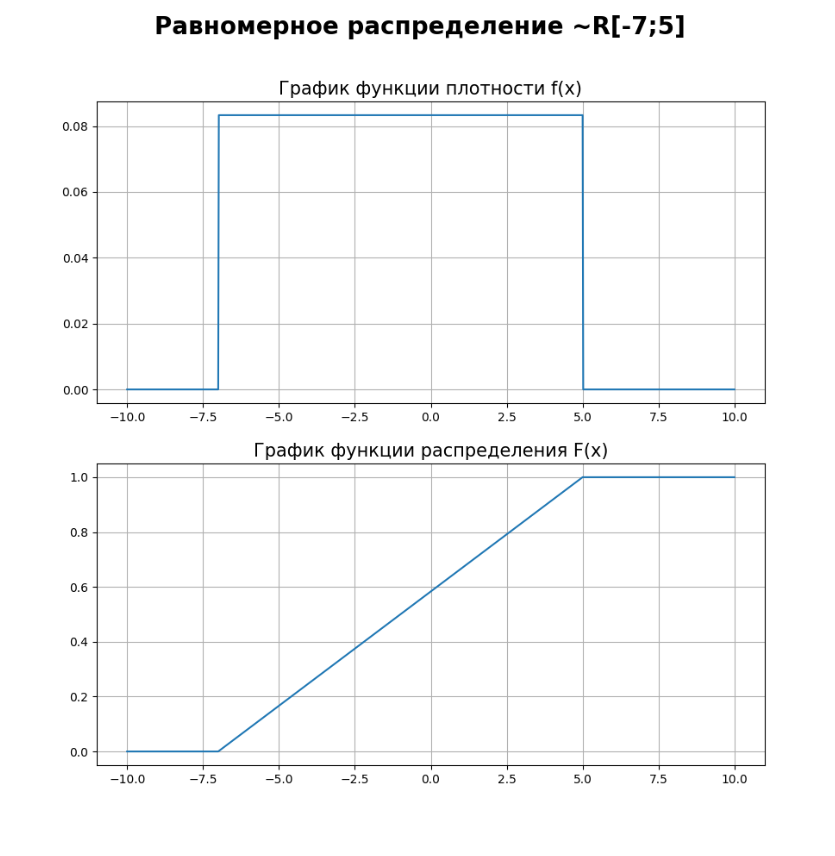
\includegraphics[width=0.6\textwidth]{img/r2.png}
	\caption{График зависимости времени выполнения запроса от количества данных всех броней}
	\label{grafics:research-2}
\end{figure}

\clearpage

\begin{table}[ht]
	\small
	\begin{center}
		\begin{threeparttable}
			\caption{Зависимость времени выполнения запроса от количества броней пользователя}
			\label{tbl:time-3}
			\begin{tabular}{|c|c|c|}
				\hline
				\multirow{2}{*}{\bfseries Количество записей в таблице броней} & \multicolumn{2}{c|}{\bfseries Время, мс} \\ \cline{2-3}
				& \bfseries Без индексов & \bfseries С индексами
				\csvreader{csv/research-3.csv}{}
				{\\\hline \csvcoli & \csvcolii & \csvcoliii } \\
				\hline
			\end{tabular}
		\end{threeparttable}
	\end{center}
\end{table}

\begin{figure}[h]
	\centering
	\includegraphics[width=0.59\textwidth]{img/r3.png}
	\caption{График зависимости времени выполнения запроса от количества броней пользователя}
	\label{grafics:research-3}
\end{figure}

\clearpage

Из результатов проведенного исследования следует, использование индекса существенно ускоряет выполнение запроса 3, который явно указывает значение искомого поля. Это приводит к значительному сокращению времени выполнения запроса, иногда более чем в десятки раз, но не всегда использование индекса приводит к таким результатам. Таким образом, время выполнения для запроса 1, где для зон включены данные пакетов и инвентаря, использование индекса снижает время выполнения в 1,15 раза.
В случае запроса 2 различия значений времени выполнения с использованием индекса и без него схожи, из чего следует что в данном случае использование индекса не улучшает время запроса.

\section*{Вывод}

В данном разделе было проведено исследование направленное на анализ влияния наличия индекса в базе данных на время выполнения запросов на получения данных из соответствующих таблиц базы данных.

Из результатов исследования следует, что воздействие индекса на время выполнения запроса в базе данных зависит от структуры самого запроса. 
Важно отметить, что использование индекса может как улучшать, так и ухудшать время выполнения, и также существуют сценарии, когда индекс не оказывает заметного влияния на время выполнения запроса.
Важно отметить, что во всех случаях использование индекса приводит к увеличению объема занимаемой памяти и увеличивает время операций вставки, изменения и удаления данных.